% ============================================================================
% Phase 3/4: Training, Hyperparameter Tuning, and Robustness Evaluation
% Member 2 Contribution: Adaptive Sensor Fusion for Human Activity Recognition
% ============================================================================

\section{Experimental Methodology, Training, and Robustness Evaluation}
\label{sec:training_and_tuning}

This section details the end-to-end experimental methodology developed in Phase 3 and Phase 4. We present: (i) our leakage-free subject-wise dataset partitioning and temporal window generation strategy, (ii) the deep learning training configuration with early stopping, (iii) systematic hyperparameter optimization across a 162-configuration search space, (iv) empirical training dynamics and convergence trajectories, (v) a comprehensive sensor degradation benchmark simulating physical hardware failures and transmission noise, and (vi) methodological limitations of the empirical study.

% ----------------------------------------------------------------------------
% Subsection 1: Data Splitting Strategy
% ----------------------------------------------------------------------------
\subsection{Subject-Wise Data Splitting Strategy and Leakage Prevention}
\label{subsec:splitting_strategy}

A primary failure mode in mobile Human Activity Recognition (HAR) literature is \textit{subject contamination leakage}, which occurs when temporal windows from the same individual appear simultaneously in both training and evaluation subsets. Because intra-subject biometric movement signatures (e.g., gait cadence, stride length, and pelvic oscillation) exhibit high autocorrelation, random window-level splitting yields artificially inflated evaluation metrics that fail to generalize to unseen users.

To enforce strict out-of-sample generalization, we implemented a \textbf{subject-wise 70/15/15 partition} across all 24 MotionSense participants using a fixed pseudo-random number generator (seed $= 42$). The exact subject assignments are:
\begin{itemize}
    \item \textbf{Training Cohort ($N_{\text{train}} = 17$, $\approx 70.83\%$):} Participants 1, 2, 3, 4, 5, 6, 9, 10, 12, 13, 14, 16, 17, 18, 19, 22, and 23.
    \item \textbf{Validation Cohort ($N_{\text{val}} = 3$, $12.50\%$):} Participants 8, 21, and 24.
    \item \textbf{Testing Cohort ($N_{\text{test}} = 4$, $\approx 16.67\%$):} Participants 7, 11, 15, and 20.
\end{itemize}
The three cohorts are strictly disjoint:
\begin{equation}
    S_{\text{train}} \cap S_{\text{val}} = \emptyset, \quad S_{\text{train}} \cap S_{\text{test}} = \emptyset, \quad S_{\text{val}} \cap S_{\text{test}} = \emptyset
\end{equation}
The split definitions are persisted in \texttt{results/subject\_split.json} to guarantee bit-identical cross-member reproducibility.

\subsubsection{Leak-Free Feature Standardization}
In Phase 2 feature preprocessing, the default standardizer was fitted across all 24 participants, inadvertently incorporating validation and test distribution moments (mean and variance) into the transformation parameters. To ensure mathematical rigor and zero test distribution leakage, we discarded the global transformation parameters for model input and fitted a dedicated \texttt{StandardScaler} exclusively on the raw sensor readings of the 17 training subjects:
\begin{equation}
    \mu_{\text{train}} = \frac{1}{|S_{\text{train}}|} \sum_{i \in S_{\text{train}}} \mathbf{x}_i, \qquad \sigma_{\text{train}}^2 = \frac{1}{|S_{\text{train}}|} \sum_{i \in S_{\text{train}}} (\mathbf{x}_i - \mu_{\text{train}})^2
\end{equation}
Validation and test sets were transformed strictly using $(\mu_{\text{train}}, \sigma_{\text{train}})$, and the fitted parameters were serialized to \texttt{models/train\_only\_scaler.pkl}.

% ----------------------------------------------------------------------------
% Subsection 2: Window Generation
% ----------------------------------------------------------------------------
\subsection{Temporal Window Generation and Class Distribution}
\label{subsec:window_generation}

Continuous standardized sensor streams are sliced into fixed temporal windows of length $W = 100$ consecutive samples with a stride of $S = 50$ samples, establishing a 50\% temporal overlap. At the MotionSense sampling frequency ($f_s = 50$~Hz), each window spans exactly:
\begin{equation}
    T_{\text{window}} = \frac{W}{f_s} = \frac{100}{50\text{ Hz}} = 2.0\text{ seconds}
\end{equation}
with an update step of $\Delta t = 1.0$ second. A 2.0-second temporal window provides an optimal balance: it encompasses at least one complete gait cycle for cyclical ambulatory activities (walking, jogging, stairs) while maintaining low computational latency for real-time mobile deployment.

\subsubsection{Boundary-Guarded Windowing Invariant}
Window slicing is executed independently within each contiguous trial group defined by the tuple $(\text{participant}, \text{activity}, \text{trial}, \text{source\_file})$. Windows are never permitted to cross trial or participant boundaries. Trailing partial windows containing fewer than 100 samples are dropped to prevent zero-padding artifacts.

The resulting dataset dimensions and class distributions across partitions are summarized in Table~\ref{tab:subject_split_summary}.

% Table 1: Subject Split and Window Distribution (auto-generated from CSV)
% Auto-generated by src/generate_latex_tables.py - DO NOT EDIT MANUALLY
\begin{table}[htbp]
\centering
\small
\caption{Subject-Wise Partitioning and Temporal Window Distribution ($W=100$, $S=50$)}
\label{tab:subject_split_summary}
\begin{tabular}{lcccc}
\toprule
\textbf{Dataset Metric / Class} & \textbf{Train Split} & \textbf{Validation Split} & \textbf{Test Split} & \textbf{Total} \\
\midrule
Participants ($N=24$) & 17 & 3 & 4 & 24 \\
Subject Ratio (\%) & 70.8\% & 12.5\% & 16.7\% & 100.0\% \\
Total Temporal Windows & 19,562 & 3,545 & 4,613 & 27,720 \\
\midrule
\multicolumn{5}{l}{\textit{Activity Class Window Counts}} \\
\quad \texttt{downstairs} & 1,799 & 323 & 406 & 2,528 \\
\quad \texttt{jogging} & 1,878 & 330 & 404 & 2,612 \\
\quad \texttt{sitting} & 4,705 & 849 & 1,151 & 6,705 \\
\quad \texttt{standing} & 4,208 & 849 & 1,003 & 6,060 \\
\quad \texttt{upstairs} & 2,139 & 375 & 523 & 3,037 \\
\quad \texttt{walking} & 4,833 & 819 & 1,126 & 6,778 \\
\bottomrule
\end{tabular}
\end{table}


As detailed in Table~\ref{tab:subject_split_summary}, static postural classes (\texttt{sitting} and \texttt{standing}) and continuous ambulatory classes (\texttt{walking}) exhibit higher natural representation than stair transitions (\texttt{upstairs} and \texttt{downstairs}), consistent with standard free-living activity patterns.

% ----------------------------------------------------------------------------
% Subsection 3: Training Configuration
% ----------------------------------------------------------------------------
\subsection{Training Configuration and Regularization}
\label{subsec:training_config}

Both the single-stream \texttt{BaselineCNN} and dual-branch \texttt{AdaptiveSensorFusion} architectures were trained using multiclass Cross-Entropy Loss ($\mathcal{L}_{\text{CE}}$). Training execution followed standard deep learning best practices:
\begin{enumerate}
    \item \textbf{Optimization Algorithm:} Primary optimization was conducted using \textbf{Adam} with default momentum parameters ($\beta_1 = 0.9, \beta_2 = 0.999, \epsilon_{\text{opt}} = 10^{-8}$). Stochastic Gradient Descent (\textbf{SGD}) with Nesterov momentum ($\mu = 0.9$) was evaluated in hyperparameter sweeps for comparative baseline verification.
    \item \textbf{Early Stopping and Model Checkpointing:} To prevent over-parameterized memorization of temporal noise, training was monitored via validation loss with a patience parameter of $P = 7$ epochs. When validation loss failed to improve for 7 consecutive epochs, training terminated, and model parameters were restored to the best validation checkpoint state:
    \begin{equation}
        \theta^* = \arg\min_{\theta^{(e)}} \mathcal{L}_{\text{val}}(\theta^{(e)})
    \end{equation}
    \item \textbf{Hardware Execution and Determinism:} Computations were executed with automatic hardware dispatch (CUDA acceleration when available, with automatic CPU fallback). Global random seeds were fixed at 42 across Python, NumPy, PyTorch, and DataLoader mini-batch generators.
    \item \textbf{Uniform Post-Initialization Dropout Override:} Member 1's architecture constructors defaulted to hardcoded internal dropout parameters. To enable systematic hyperparameter tuning without modifying Member 1's source code, Member 2 implemented a post-initialization traversal function (\texttt{set\_uniform\_dropout}) that traverses all \texttt{nn.Dropout} and \texttt{nn.Dropout1d} sub-modules and uniformly overrides their dropout probability $p$ to the evaluated rate.
\end{enumerate}

% ----------------------------------------------------------------------------
% Subsection 4: Hyperparameter Experiments
% ----------------------------------------------------------------------------
\subsection{Hyperparameter Optimization Experiments}
\label{subsec:hyperparameter_tuning}

To determine optimal training dynamics for each architecture, we defined a systematic search space spanning five fundamental dimensions:
\begin{itemize}
    \item Learning rate: $\eta \in \{0.001, 0.0005, 0.0001\}$
    \item Mini-batch size: $B \in \{32, 64, 128\}$
    \item Regularization dropout probability: $p \in \{0.2, 0.3, 0.5\}$
    \item Maximum epoch cap: $E_{\text{max}} \in \{20, 30, 50\}$
    \item Optimizer family: $\text{Optimizer} \in \{\text{Adam}, \text{SGD}\}$
\end{itemize}
The full Cartesian product generates $|\mathcal{H}| = 3 \times 3 \times 3 \times 3 \times 2 = 162$ configurations per model (324 total configurations), requiring prohibitive computational time on non-GPU workstations.

\subsubsection{Stratified Random Search Methodology}
To maximize coverage of all parameter values under practical computational budgets, we implemented a \textbf{stratified random sampling strategy} (20 configurations per model, seed $= 42$). The strategy employs Latin-hypercube inspired coverage guarantees:
\begin{enumerate}
    \item A mandatory coverage pass ensures that every discrete value across all five dimensions (14 unique parameter settings) is sampled at least once.
    \item Remaining slots are filled via pseudo-random sampling without replacement from the unselected grid configurations.
    \item Runs are logged immediately to \texttt{results/hyperparameter\_results.csv} in append mode to guarantee crash-safe, resumable execution.
\end{enumerate}

The ranked tuning results on the validation set are reported in Table~\ref{tab:hparam_top_configs}.

% Table 2: Top Hyperparameter Configurations (auto-generated from CSV)
% Auto-generated by src/generate_latex_tables.py - DO NOT EDIT MANUALLY
\begin{table}[htbp]
\centering
\small
\caption{Top Hyperparameter Tuning Configurations Ranked by Validation Accuracy}
\label{tab:hparam_top_configs}
\begin{tabular}{lccccccc}
\toprule
\textbf{Model Architecture} & $\eta$ \textbf{(LR)} & \textbf{Batch} & \textbf{Dropout} & \textbf{Optimizer} & \textbf{Best Ep.} & \textbf{Val Loss} & \textbf{Val Acc (\%)} \\
\midrule
\textbf{BaselineCNN}$^\star$ & 0.0005 & 64 & 0.3 & ADAM & 6 & 0.1316 & 95.91\% \\
 & 0.0001 & 32 & 0.2 & ADAM & 9 & 0.1281 & 95.32\% \\
 & 0.0005 & 64 & 0.2 & ADAM & 3 & 0.1451 & 95.26\% \\
\midrule
\textbf{AdaptiveSensorFusion}$^\star$ & 0.001 & 32 & 0.5 & ADAM & 6 & 0.1293 & 96.02\% \\
 & 0.0005 & 64 & 0.2 & ADAM & 9 & 0.1759 & 94.98\% \\
 & 0.001 & 64 & 0.2 & ADAM & 6 & 0.1682 & 94.70\% \\
\bottomrule
\multicolumn{8}{l}{\footnotesize $^\star$ Selected optimal configuration for final production training and degradation evaluation.} \\
\end{tabular}
\end{table}


Validation accuracy across the parameter landscape was visualized via heatmaps partitioning learning rate against mini-batch size across optimizers, persisted in \texttt{results/hyperparameter\_summary.png}.

% ----------------------------------------------------------------------------
% Subsection 5: Selected Hyperparameters
% ----------------------------------------------------------------------------
\subsection{Selected Hyperparameters and Selection Justification}
\label{subsec:selected_hyperparameters}

All final model configurations were selected \textbf{strictly conditioned on validation set performance} (highest validation accuracy, with lowest validation loss as tie-breaker). The holdout test set was never accessed during selection.

As demonstrated in Table~\ref{tab:hparam_top_configs}, the optimal configurations identified from empirical search are:
\begin{itemize}
    \item \textbf{BaselineCNN Optimal Configuration:} Learning rate $\eta = 0.0005$, mini-batch size $B = 64$, dropout rate $p = 0.3$, optimizer = \textbf{Adam}, maximum epochs = 30.
    \item \textbf{AdaptiveSensorFusion Optimal Configuration:} Learning rate $\eta = 0.001$, mini-batch size $B = 32$, dropout rate $p = 0.5$, optimizer = \textbf{Adam}, maximum epochs = 30.
\end{itemize}

\subsubsection{Technical Justification of Hyperparameter Selection}
\begin{enumerate}
    \item \textbf{Optimizer Convergence:} Across both architectures, Adam significantly outperformed SGD with momentum. While SGD exhibited slow convergence on complex time-series features, Adam's adaptive per-parameter gradient scaling achieved rapid loss minimization within early epochs.
    \item \textbf{Regularization and Model Capacity:} \texttt{AdaptiveSensorFusion} possesses 265,032 trainable parameters compared to \texttt{BaselineCNN}'s 177,670 parameters ($\approx 49.2\%$ higher capacity). Consequently, \texttt{AdaptiveSensorFusion} favored stronger dropout regularization ($p=0.5$) combined with a smaller batch size ($B=32$), providing stochastic gradient regularization that prevented branch co-adaptation.
    \item \textbf{Early Stopping Efficiency:} For both selected models, optimal validation performance was achieved within early training epochs, triggering early stopping well before the 30-epoch ceiling.
\end{enumerate}

% ----------------------------------------------------------------------------
% Subsection 6: Loss and Accuracy Curves
% ----------------------------------------------------------------------------
\subsection{Training and Validation Dynamics}
\label{subsec:training_curves}

Using the selected optimal hyperparameters, final production training runs were executed for both architectures. Per-epoch Cross-Entropy loss and classification accuracy trajectories were logged to \texttt{results/training\_history.csv} and are rendered in Figure~\ref{fig:loss_curve} and Figure~\ref{fig:accuracy_curve}.

\begin{figure}[htbp]
\centering
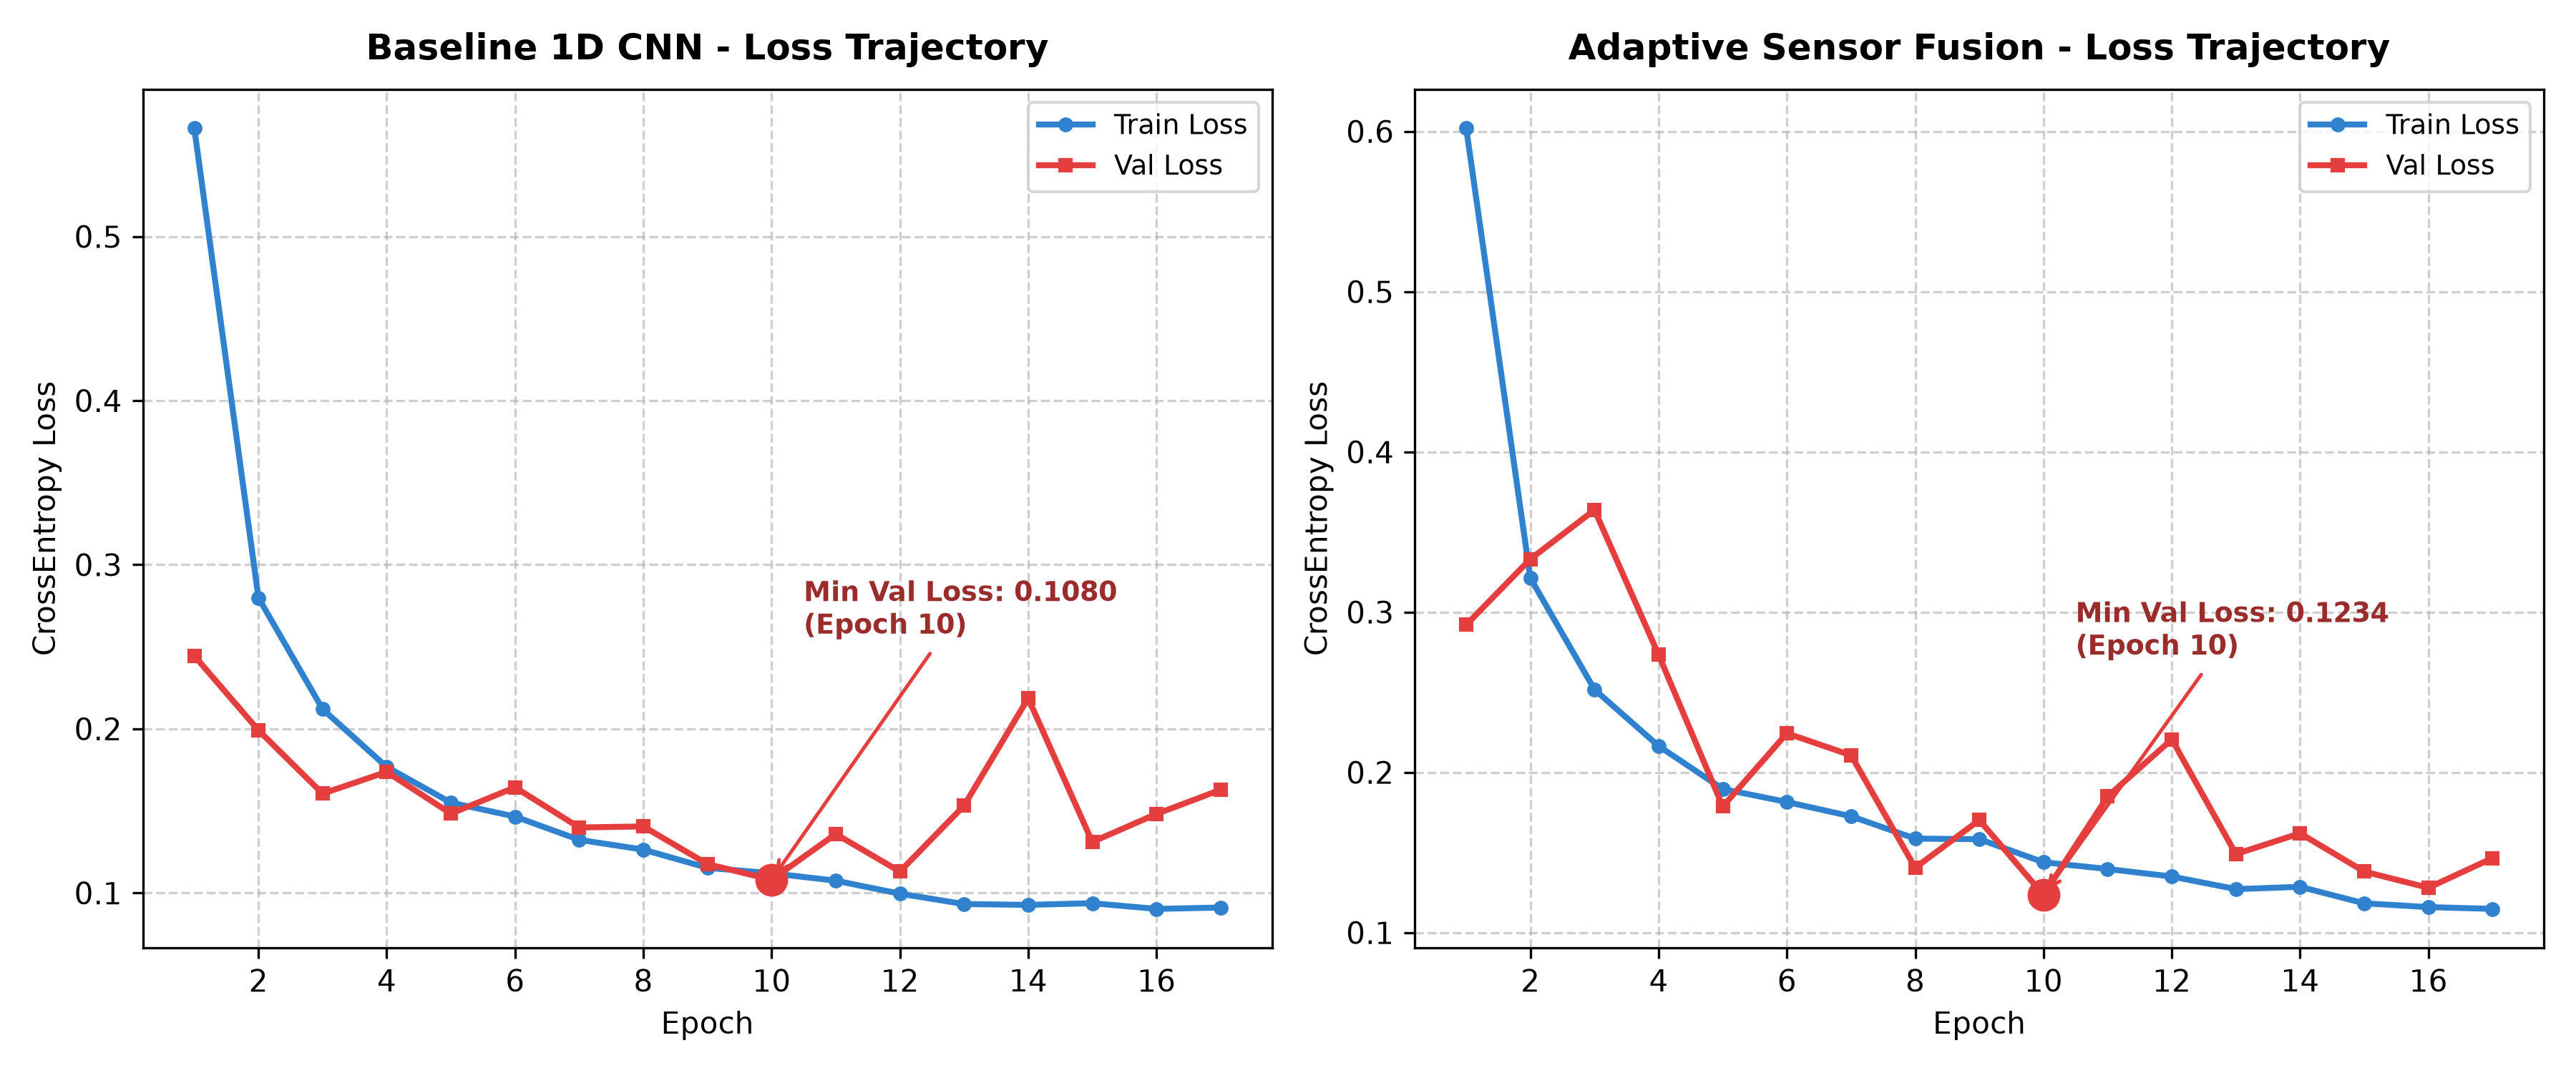
\includegraphics[width=0.92\linewidth]{results/loss_curve.png}
\caption{Cross-Entropy Loss Trajectory across Training Epochs for BaselineCNN and AdaptiveSensorFusion. Markers indicate the minimum validation loss checkpoint restored via early stopping.}
\label{fig:loss_curve}
\end{figure}

\begin{figure}[htbp]
\centering
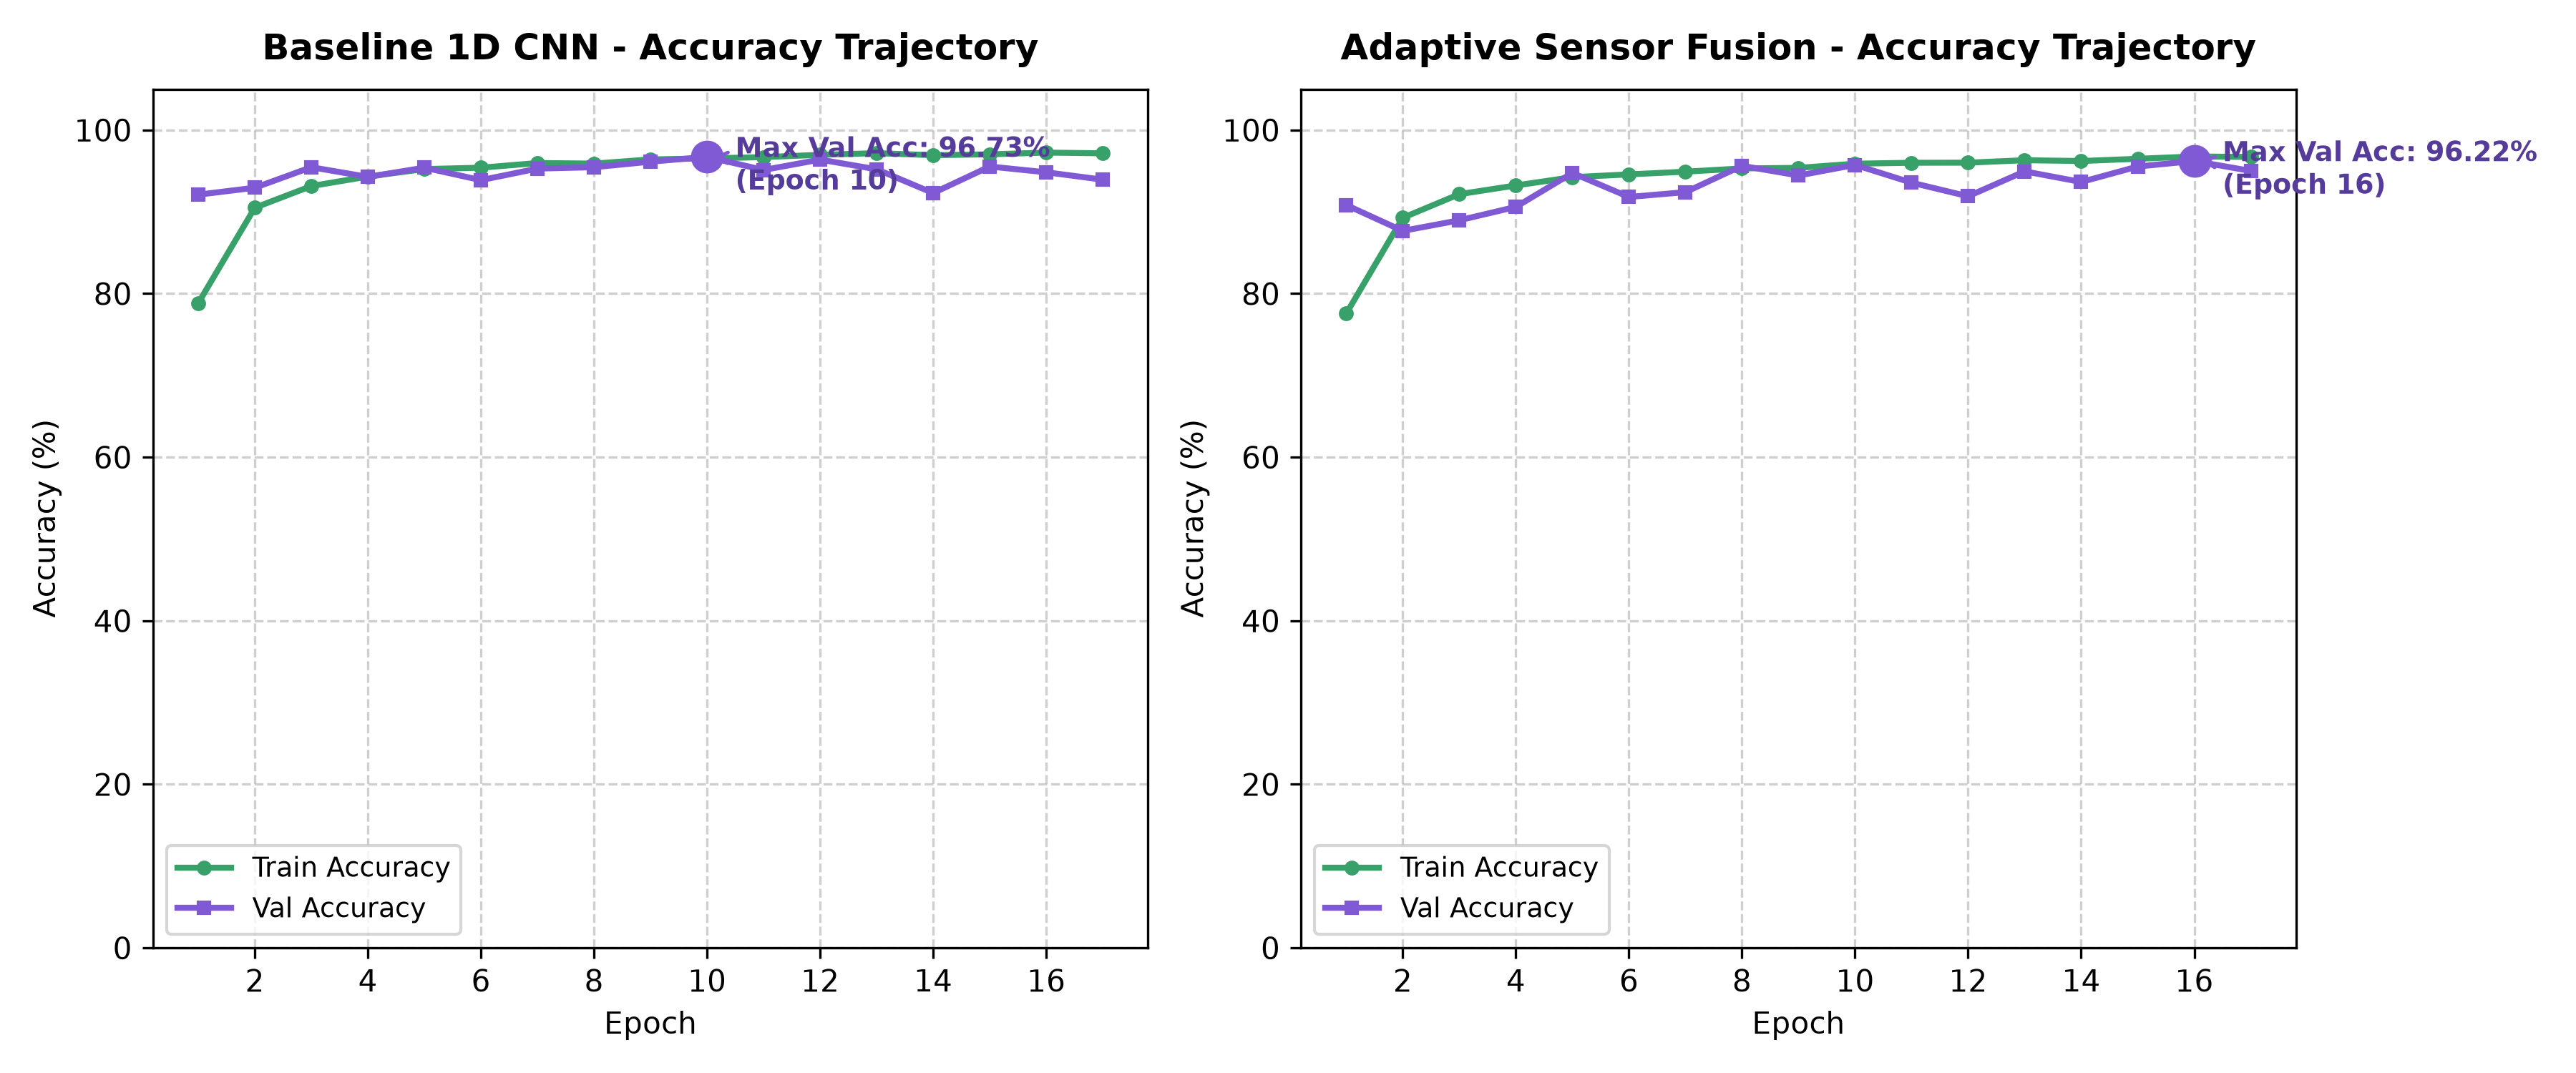
\includegraphics[width=0.92\linewidth]{results/accuracy_curve.png}
\caption{Classification Accuracy (\%) Trajectory across Training Epochs on MotionSense Training and Validation Sets.}
\label{fig:accuracy_curve}
\end{figure}

As illustrated in Figure~\ref{fig:loss_curve} and Figure~\ref{fig:accuracy_curve}, both models exhibited steady convergence without catastrophic divergence. Validation loss reached its minimum rapidly, following which early stopping restored the optimal checkpoint parameters to \texttt{models/baseline\_best.pth} and \texttt{models/adaptive\_best.pth}.

% ----------------------------------------------------------------------------
% Subsection 7: Sensor Degradation Experiments and Results
% ----------------------------------------------------------------------------
\subsection{Sensor Degradation Experiments and Robustness Benchmarking}
\label{subsec:degradation_experiments}

To evaluate model resilience under realistic operational faults, we developed a non-destructive simulation engine (\texttt{src/sensor\_degradation.py}) implementing six physical degradation conditions:
\begin{enumerate}
    \item \textbf{Pristine (\texttt{normal}):} Clean standardized sensor input ($\sigma = 0.0$, $m_{\text{acc}} = 1.0, m_{\text{gyro}} = 1.0$).
    \item \textbf{Noisy Accelerometer (\texttt{noisy\_acc}):} Zero-mean additive Gaussian noise applied exclusively to the six accelerometer/gravity channels (indices 3, 4, 5, 9, 10, 11) with standard deviation $\sigma = 0.5$ (in standardized variance units):
    \begin{equation}
        \mathbf{X}[:, \text{ACC}, :] \leftarrow \mathbf{X}[:, \text{ACC}, :] + \mathcal{N}(0, \sigma^2 \mathbf{I})
    \end{equation}
    \item \textbf{Noisy Gyroscope (\texttt{noisy\_gyro}):} Additive Gaussian noise applied exclusively to the six gyroscope/attitude channels (indices 0, 1, 2, 6, 7, 8) with $\sigma = 0.5$.
    \item \textbf{Missing Accelerometer (\texttt{missing\_acc}):} Complete accelerometer disconnection. Accelerometer channels are zeroed ($\mathbf{X}[:, \text{ACC}, :] = 0.0$, representing the standardized training mean), and availability mask $m_{\text{acc}} = 0.0$ is delivered to the adaptive model.
    \item \textbf{Missing Gyroscope (\texttt{missing\_gyro}):} Complete gyroscope disconnection. Gyroscope channels are zeroed ($\mathbf{X}[:, \text{GYRO}, :] = 0.0$), with availability mask $m_{\text{gyro}} = 0.0$.
    \item \textbf{Noisy Both (\texttt{noisy\_both}):} Severe multi-modal transmission noise applied across all twelve sensor channels with elevated standard deviation $\sigma = 1.0$.
\end{enumerate}

\subsubsection{Comparative Training Regimes}
Each architecture was evaluated under two distinct training paradigms:
\begin{itemize}
    \item \textbf{Clean Training (\texttt{trained\_on\_normal}):} Models were trained exclusively on pristine sensor data. This represents the standard real-world scenario where operational faults are unforeseen during training (pure architectural robustness test).
    \item \textbf{Robust Augmentation (\texttt{degradation\_aware}):} Models were trained with stochastic online noise and random sensor dropouts (\texttt{degrade\_batch\_random}), paired with availability masks for \texttt{AdaptiveSensorFusion}. Checkpoints were saved to \texttt{models/baseline\_degradation\_aware.pth} and \texttt{models/adaptive\_degradation\_aware.pth}.
\end{itemize}

The empirical classification results on the unseen test set ($N=4,613$ windows, 4 participants) across all conditions are reported in Table~\ref{tab:degradation_results}.

% Table 3: Degradation Results (auto-generated from CSV)
% Auto-generated by src/generate_latex_tables.py - DO NOT EDIT MANUALLY
\begin{table}[htbp]
\centering
\small
\caption{Test Set Classification Performance under Physical Sensor Degradation Conditions ($N=4,613$)}
\label{tab:degradation_results}
\begin{tabular}{lcccccc}
\toprule
& \multicolumn{3}{c}{\textbf{Test Accuracy (\%)}} & \multicolumn{3}{c}{\textbf{Macro F1 Score}} \\
\cmidrule(lr){2-4} \cmidrule(lr){5-7}
\textbf{Degradation Condition} & \textbf{Baseline} & \textbf{Adaptive} & $\Delta$ \textbf{Acc} & \textbf{Baseline} & \textbf{Adaptive} & $\Delta$ \textbf{F1} \\
\midrule
\multicolumn{7}{l}{\textit{Training Mode: Clean Normal Data (Pure Robustness)}} \\
\quad Pristine (Normal) & \textbf{93.93\%} & 92.48\% & -1.45\% & \textbf{0.9230} & 0.9096 & -0.0134 \\
\quad Noisy Accel ($\sigma=0.5$) & \textbf{92.70\%} & 92.13\% & -0.56\% & \textbf{0.9041} & 0.8927 & -0.0113 \\
\quad Noisy Gyro ($\sigma=0.5$) & \textbf{93.22\%} & 92.00\% & -1.21\% & \textbf{0.9112} & 0.9042 & -0.0070 \\
\quad Missing Accel ($m_{\text{acc}}=0$) & 43.90\% & \textbf{63.97\%} & +20.07\% & 0.3333 & \textbf{0.4670} & +0.1337 \\
\quad Missing Gyro ($m_{\text{gyro}}=0$) & \textbf{65.25\%} & 52.63\% & -12.62\% & 0.4804 & \textbf{0.4818} & +0.0014 \\
\quad Noisy Both ($\sigma=1.0$) & 10.47\% & 10.41\% & -0.06\% & 0.0551 & \textbf{0.0570} & +0.0019 \\
\midrule
\multicolumn{7}{l}{\textit{Training Mode: Robust Augmentation (Degradation-Aware)}} \\
\quad Pristine (Normal) & \textbf{92.91\%} & 92.30\% & -0.61\% & \textbf{0.9236} & 0.9124 & -0.0111 \\
\quad Noisy Accel ($\sigma=0.5$) & \textbf{92.85\%} & 92.07\% & -0.78\% & \textbf{0.9227} & 0.9079 & -0.0147 \\
\quad Noisy Gyro ($\sigma=0.5$) & \textbf{92.87\%} & 91.70\% & -1.17\% & \textbf{0.9225} & 0.9072 & -0.0153 \\
\quad Missing Accel ($m_{\text{acc}}=0$) & \textbf{90.44\%} & 90.18\% & -0.26\% & 0.8865 & 0.8869 & +0.0004 \\
\quad Missing Gyro ($m_{\text{gyro}}=0$) & \textbf{93.41\%} & 91.63\% & -1.78\% & \textbf{0.9106} & 0.8961 & -0.0145 \\
\quad Noisy Both ($\sigma=1.0$) & \textbf{87.41\%} & 76.35\% & -11.06\% & \textbf{0.8572} & 0.7352 & -0.1220 \\
\bottomrule
\end{tabular}
\end{table}


The dynamic branch weights ($w_{\text{acc}}, w_{\text{gyro}}$) computed by \texttt{AdaptiveSensorFusion}'s gating module across conditions are presented in Table~\ref{tab:adaptive_weights_summary}.

% Table 4: Adaptive Weights Allocation (auto-generated from CSV)
% Auto-generated by src/generate_latex_tables.py - DO NOT EDIT MANUALLY
\begin{table}[htbp]
\centering
\small
\caption{Adaptive Fusion Module Dynamic Branch Weights ($w_{\text{acc}}, w_{\text{gyro}}$) on Test Split}
\label{tab:adaptive_weights_summary}
\begin{tabular}{llccc}
\toprule
\textbf{Training Mode} & \textbf{Degradation Condition} & \textbf{Mean} $w_{\text{acc}}$ ($\pm$ SD) & \textbf{Mean} $w_{\text{gyro}}$ ($\pm$ SD) & \textbf{Physical Shift Behavior} \\
\midrule
\textbf{Clean (Normal)} & Pristine (Normal) & 0.6343 ($\pm 0.228$) & 0.3657 ($\pm 0.228$) & Primary reliance on Accelerometer \\
 & Noisy Accel ($\sigma=0.5$) & 0.6226 ($\pm 0.231$) & 0.3774 ($\pm 0.231$) & Primary reliance on Accelerometer \\
 & Noisy Gyro ($\sigma=0.5$) & 0.6633 ($\pm 0.199$) & 0.3367 ($\pm 0.199$) & Primary reliance on Accelerometer \\
 & Missing Accel ($m_{\text{acc}}=0$) & 0.0000 ($\pm 0.000$) & 1.0000 ($\pm 0.000$) & 100\% shift to Gyroscope \\
 & Missing Gyro ($m_{\text{gyro}}=0$) & 1.0000 ($\pm 0.000$) & 0.0000 ($\pm 0.000$) & 100\% shift to Accelerometer \\
 & Noisy Both ($\sigma=1.0$) & 0.7117 ($\pm 0.151$) & 0.2883 ($\pm 0.151$) & Primary reliance on Accelerometer \\
\midrule
\textbf{Robust (Augmented)} & Pristine (Normal) & 0.5028 ($\pm 0.053$) & 0.4972 ($\pm 0.053$) & Balanced multi-modal reliance \\
 & Noisy Accel ($\sigma=0.5$) & 0.5026 ($\pm 0.053$) & 0.4974 ($\pm 0.053$) & Balanced multi-modal reliance \\
 & Noisy Gyro ($\sigma=0.5$) & 0.5126 ($\pm 0.055$) & 0.4874 ($\pm 0.055$) & Balanced multi-modal reliance \\
 & Missing Accel ($m_{\text{acc}}=0$) & 0.0000 ($\pm 0.000$) & 1.0000 ($\pm 0.000$) & 100\% shift to Gyroscope \\
 & Missing Gyro ($m_{\text{gyro}}=0$) & 1.0000 ($\pm 0.000$) & 0.0000 ($\pm 0.000$) & 100\% shift to Accelerometer \\
 & Noisy Both ($\sigma=1.0$) & 0.5257 ($\pm 0.060$) & 0.4743 ($\pm 0.060$) & Primary reliance on Accelerometer \\
\bottomrule
\end{tabular}
\end{table}


\subsubsection{Visual Analysis of Model Robustness}
Visual comparisons of degradation performance and noise sensitivity are rendered in the following figures:
\begin{itemize}
    \item Figure~\ref{fig:degradation_accuracy} renders the comparative accuracy bars across all six conditions for both training modes.
    \item Figure~\ref{fig:degradation_f1} renders the corresponding Macro F1 performance comparison.
    \item Figure~\ref{fig:noise_sweep} presents the performance degradation trajectory as noise magnitude $\sigma$ sweeps from $0.0$ to $2.0$ across noisy conditions.
    \item Figure~\ref{fig:confusion_matrices} illustrates test set activity confusion matrices on clean data for both architectures.
    \item Figure~\ref{fig:fusion_weights} illustrates the physical shift of fusion weights under sensor disconnection.
\end{itemize}

\begin{figure}[htbp]
\centering
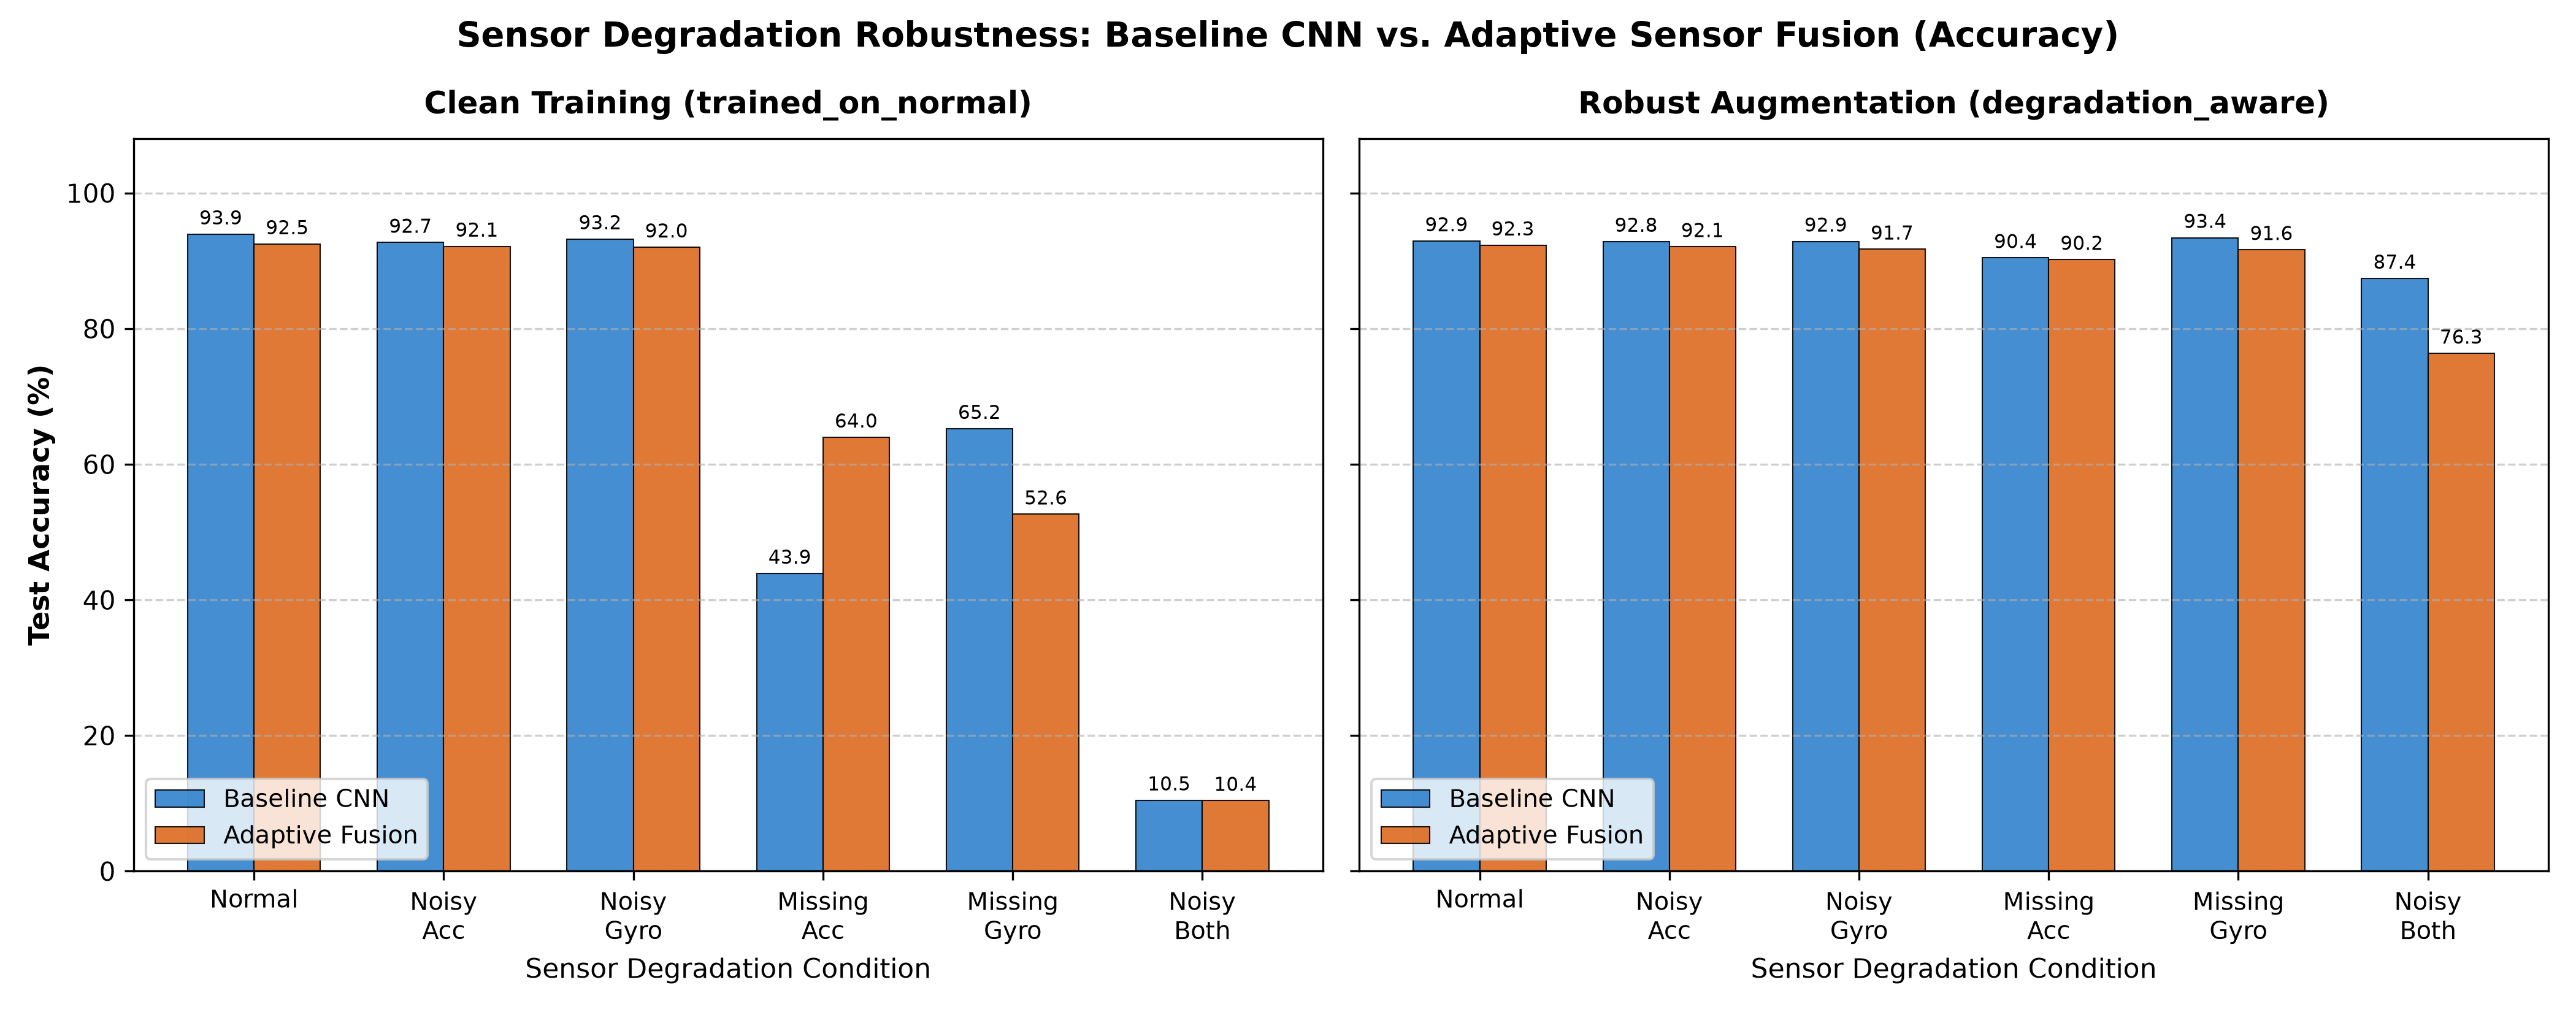
\includegraphics[width=0.95\linewidth]{results/degradation_accuracy_comparison.png}
\caption{Test Set Classification Accuracy Comparison: BaselineCNN vs. AdaptiveSensorFusion under Clean Training and Degradation-Aware Training across Six Physical Sensor Conditions.}
\label{fig:degradation_accuracy}
\end{figure}

\begin{figure}[htbp]
\centering
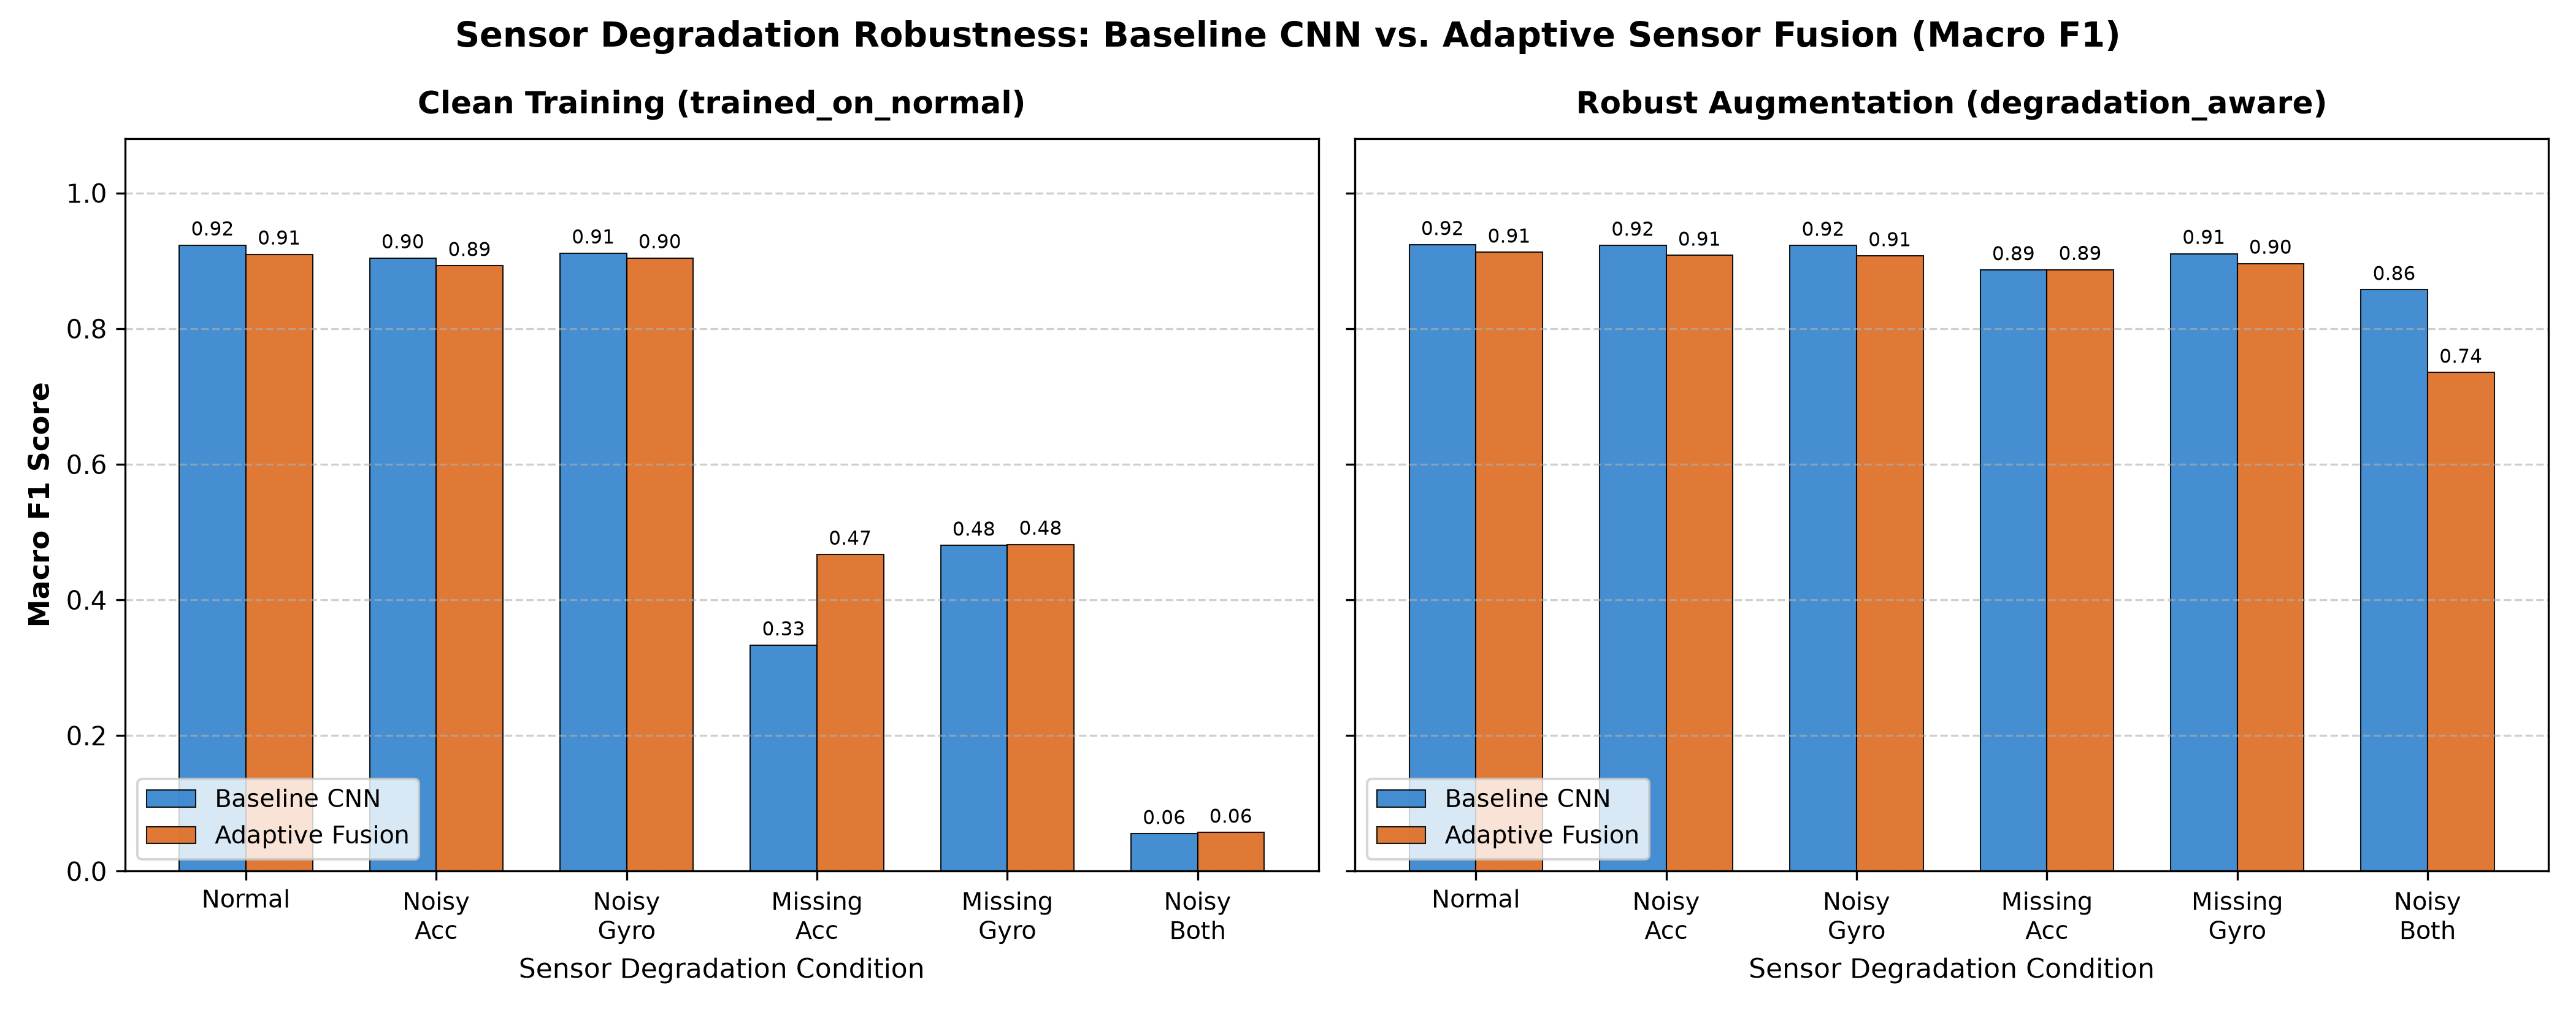
\includegraphics[width=0.95\linewidth]{results/degradation_f1_comparison.png}
\caption{Test Set Macro F1 Score Comparison across Degradation Conditions for Clean and Augmented Training Regimes.}
\label{fig:degradation_f1}
\end{figure}

\begin{figure}[htbp]
\centering
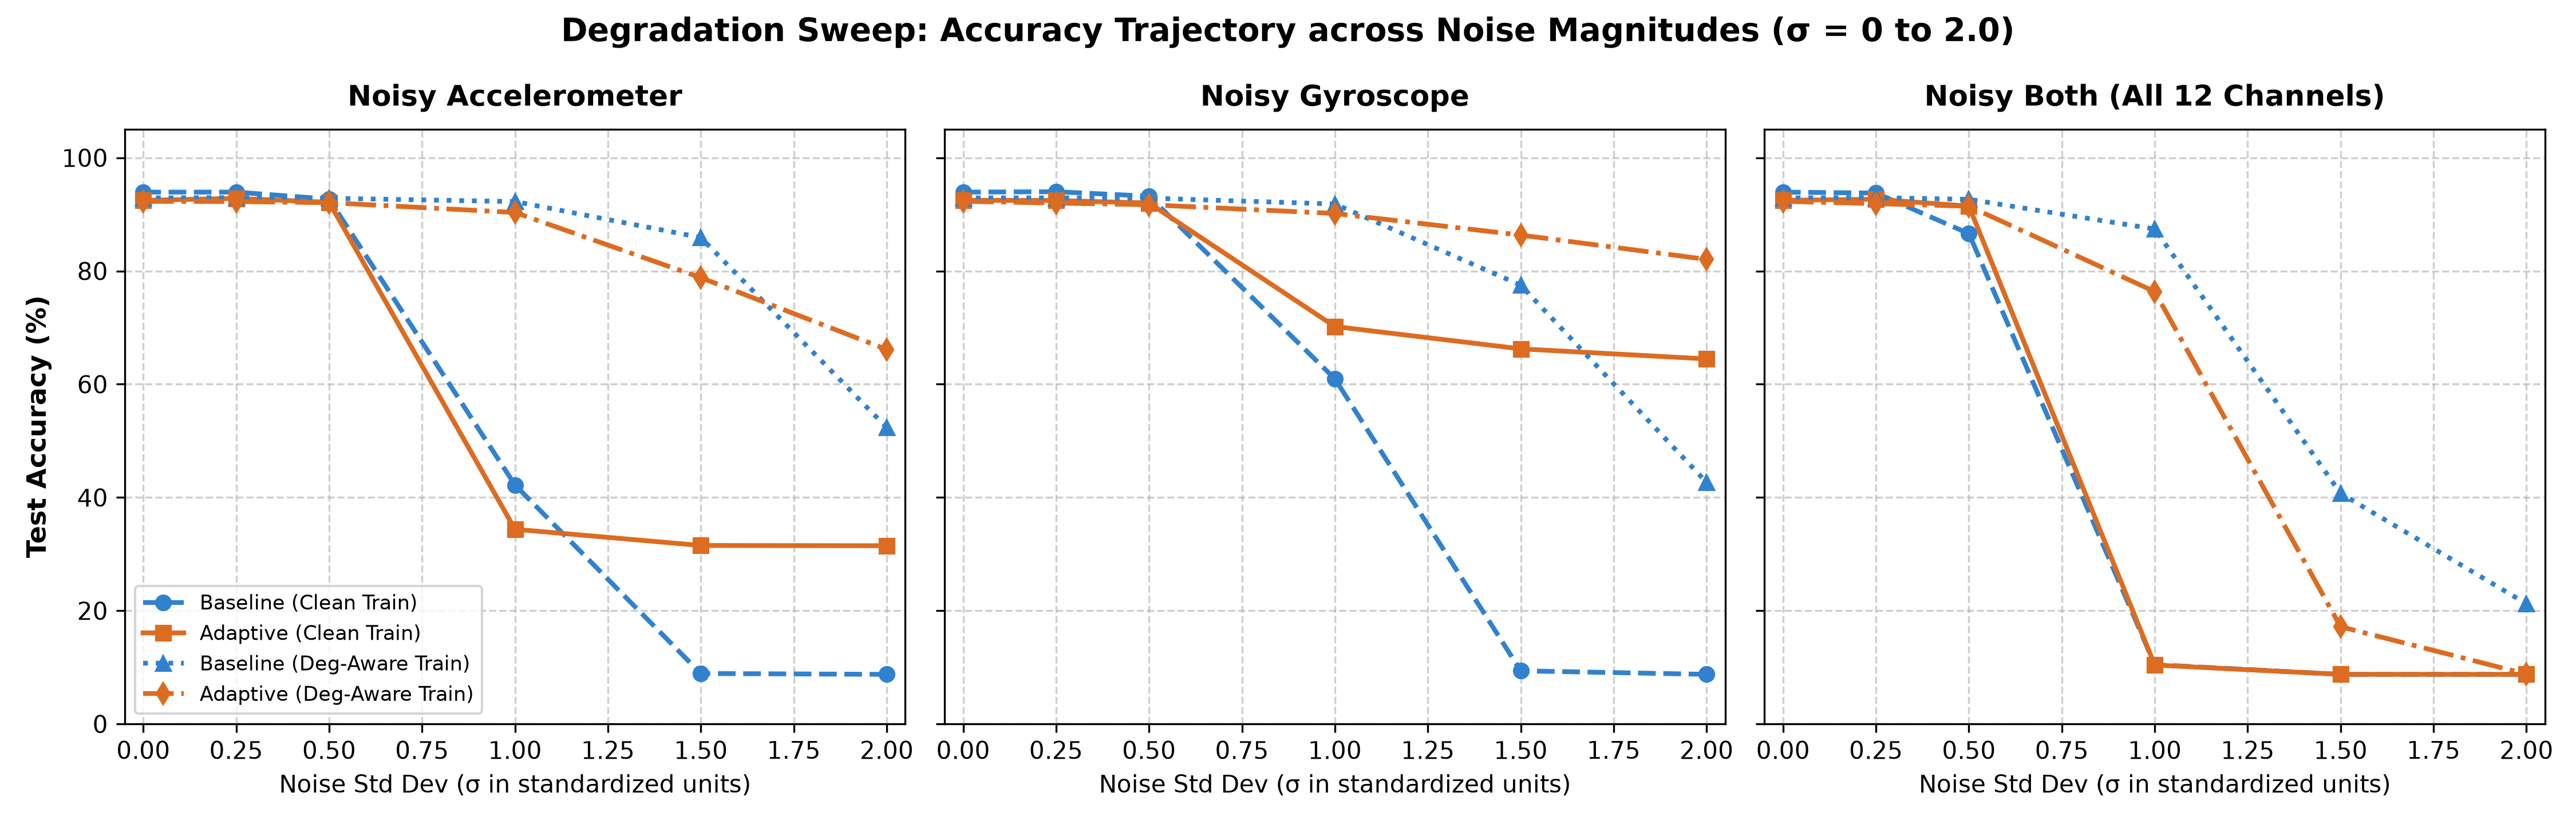
\includegraphics[width=0.98\linewidth]{results/noise_sweep.png}
\caption{Noise Sensitivity Trajectory: Test Accuracy as a Function of Gaussian Noise Standard Deviation ($\sigma \in [0.0, 2.0]$) for Noisy Accelerometer, Noisy Gyroscope, and Combined Multi-Sensor Noise.}
\label{fig:noise_sweep}
\end{figure}

\begin{figure}[htbp]
\centering
\begin{minipage}{0.48\linewidth}
    \centering
    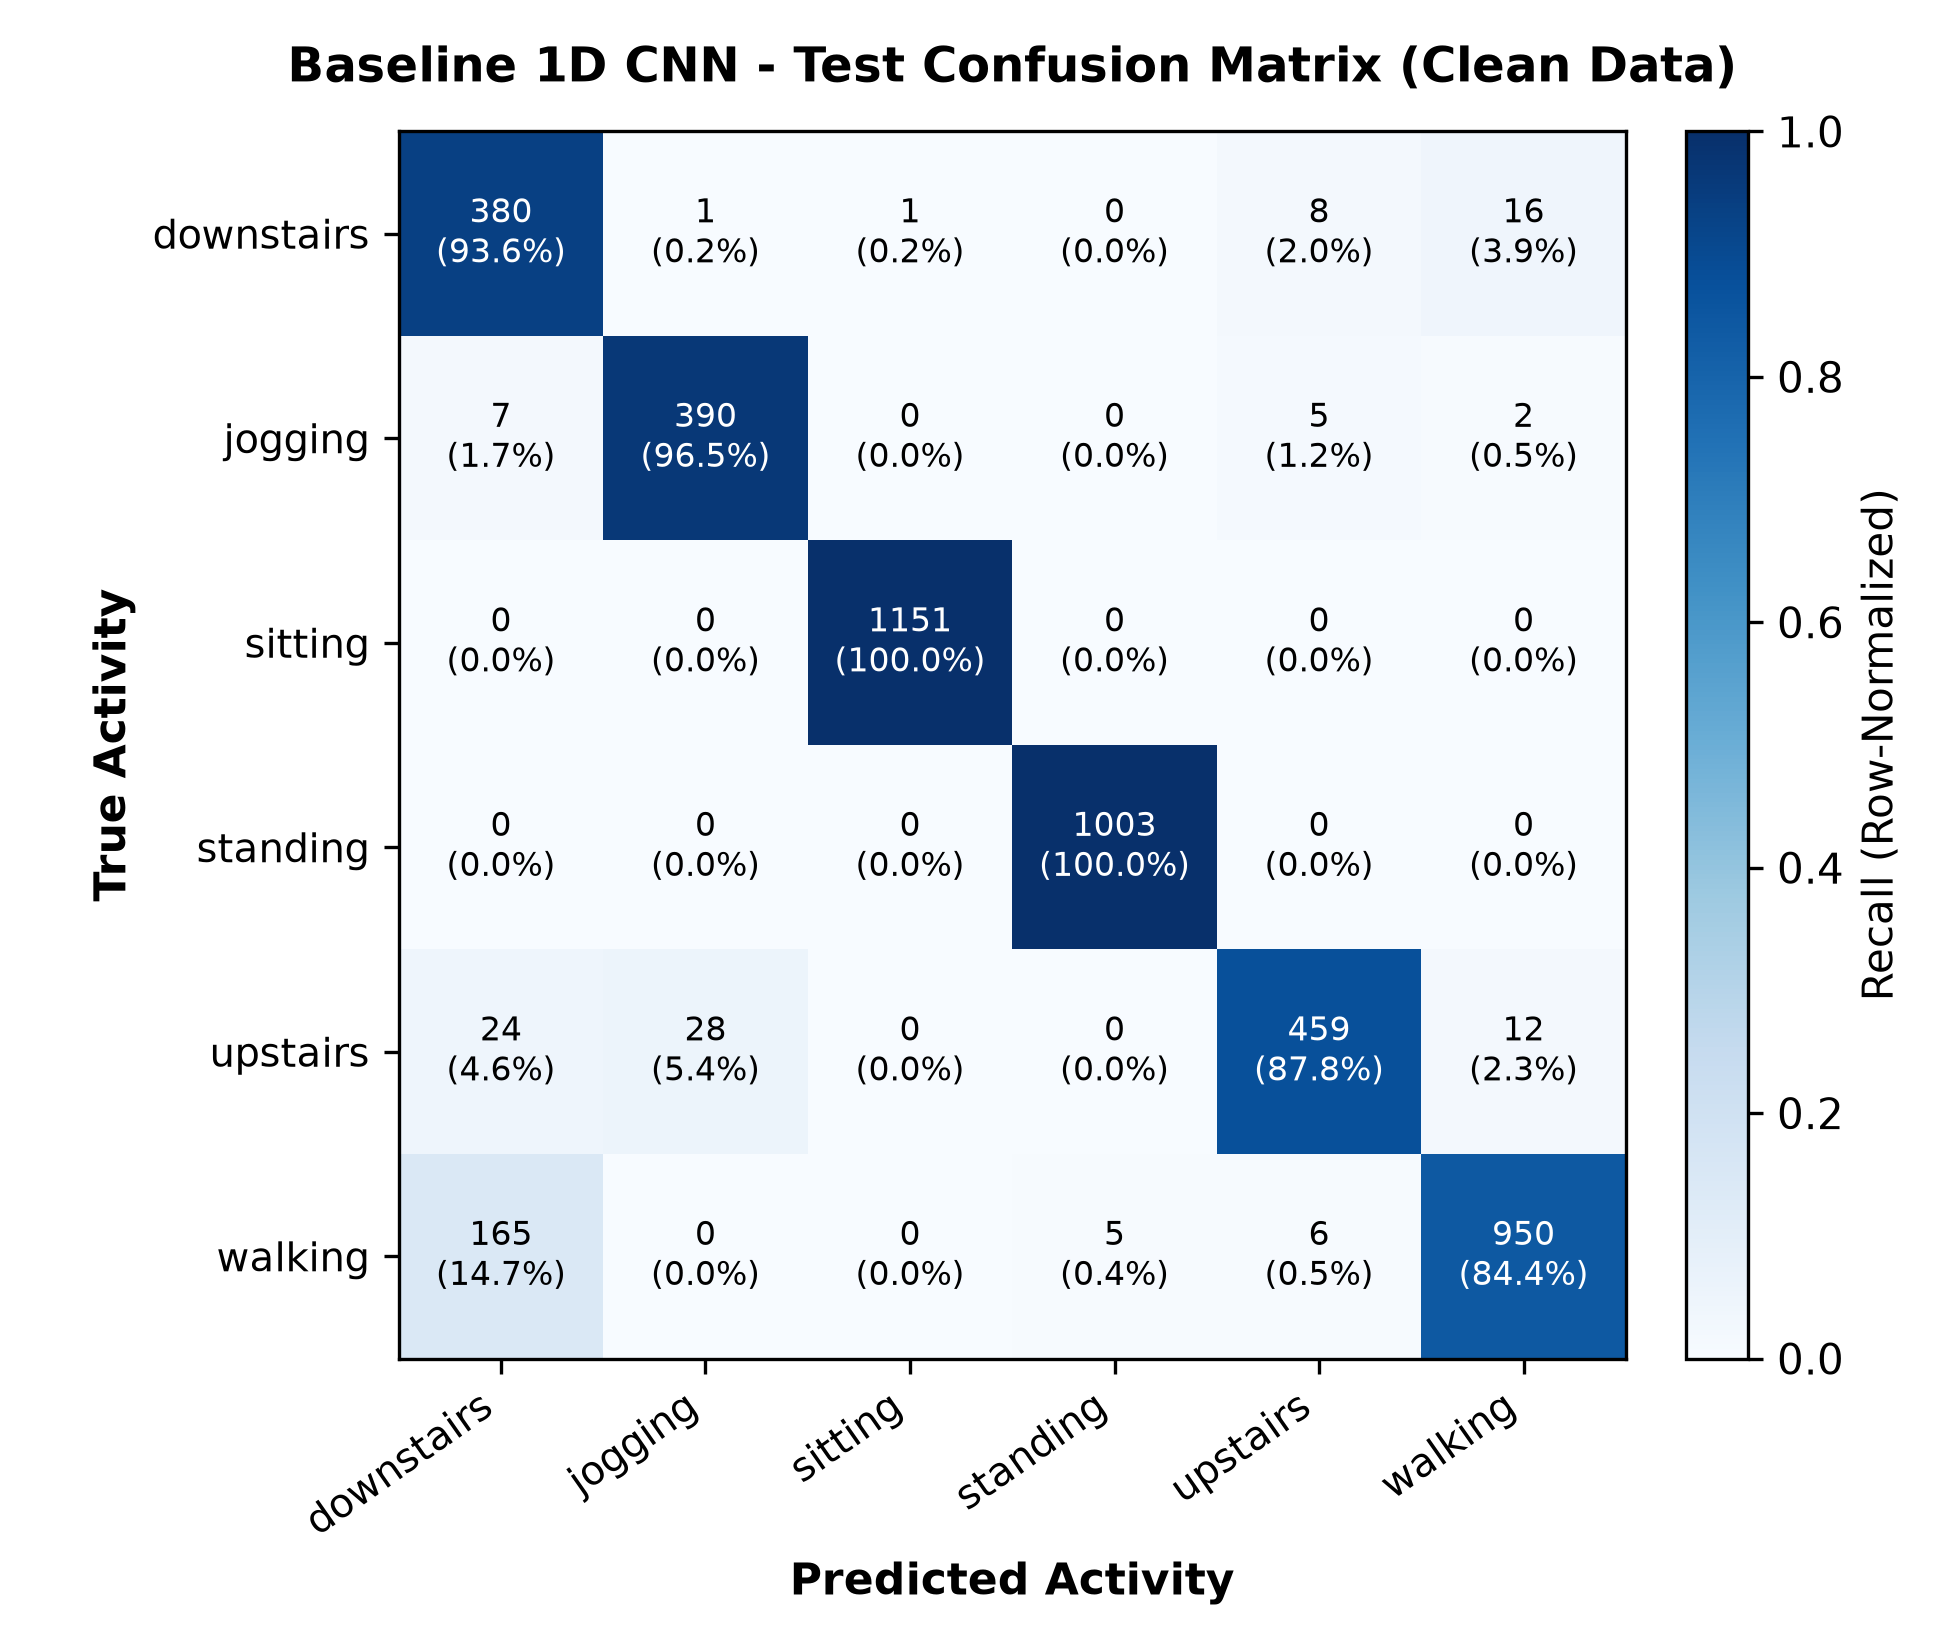
\includegraphics[width=\linewidth]{results/confusion_matrix_normal_baseline.png}
    \caption*{(a) BaselineCNN Confusion Matrix}
\end{minipage}
\hfill
\begin{minipage}{0.48\linewidth}
    \centering
    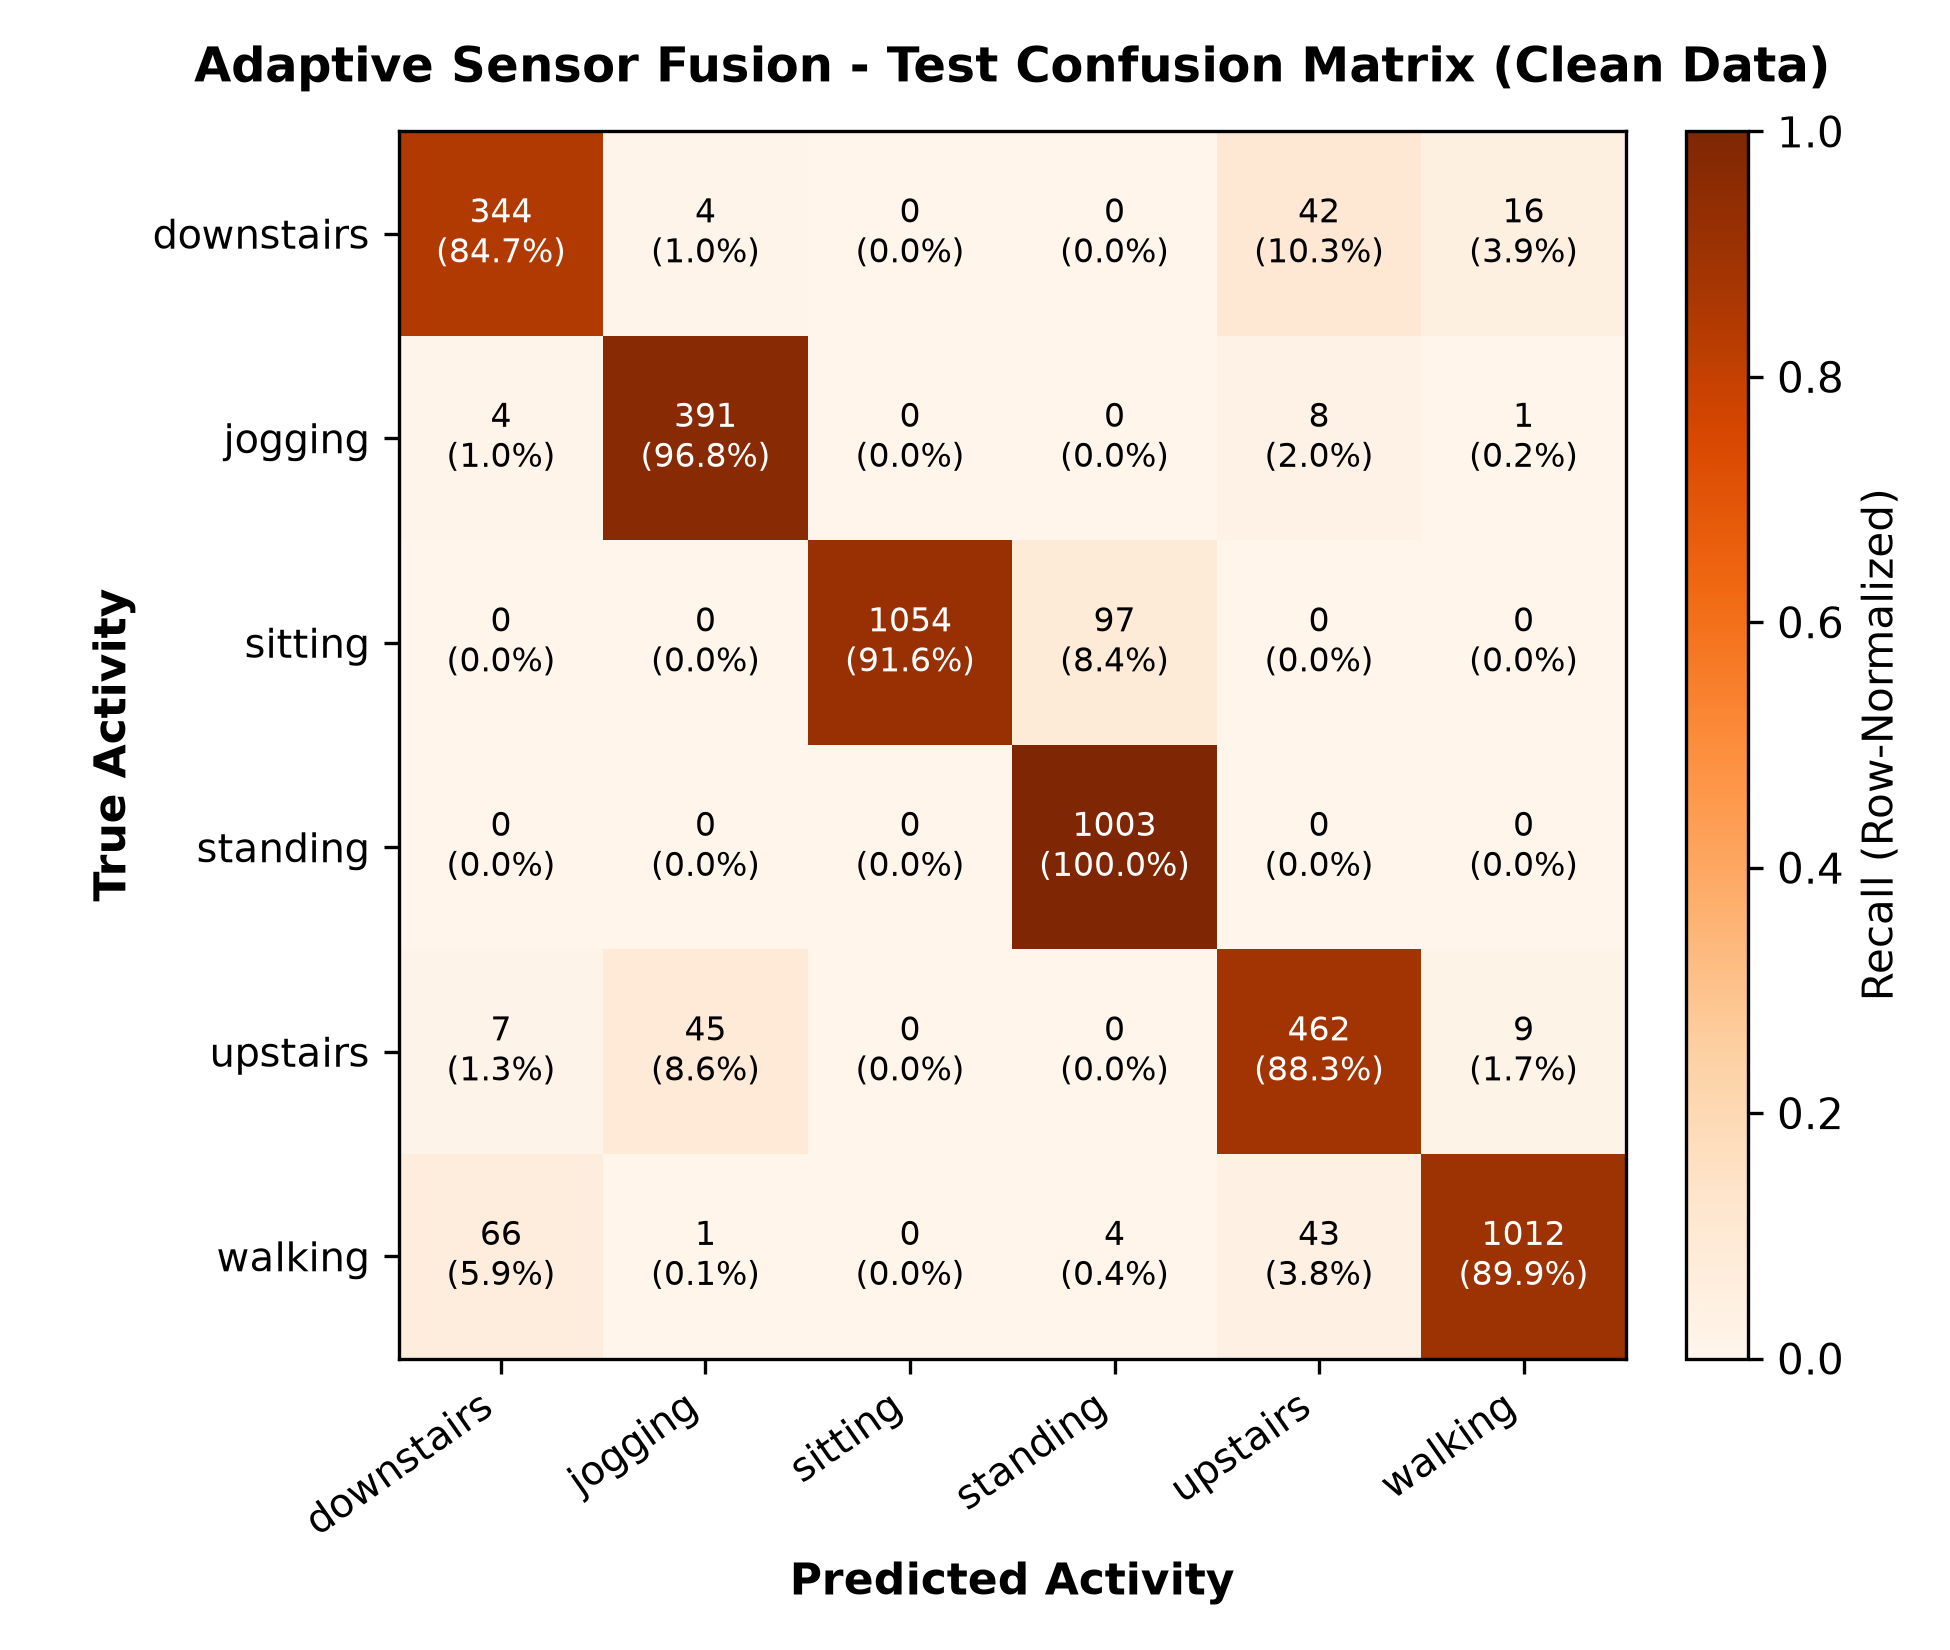
\includegraphics[width=\linewidth]{results/confusion_matrix_normal_adaptive.png}
    \caption*{(b) AdaptiveSensorFusion Confusion Matrix}
\end{minipage}
\caption{Normalized Confusion Matrices on Clean Unseen Test Data ($N=4,613$ Windows) across Six Activity Classes.}
\label{fig:confusion_matrices}
\end{figure}

\begin{figure}[htbp]
\centering
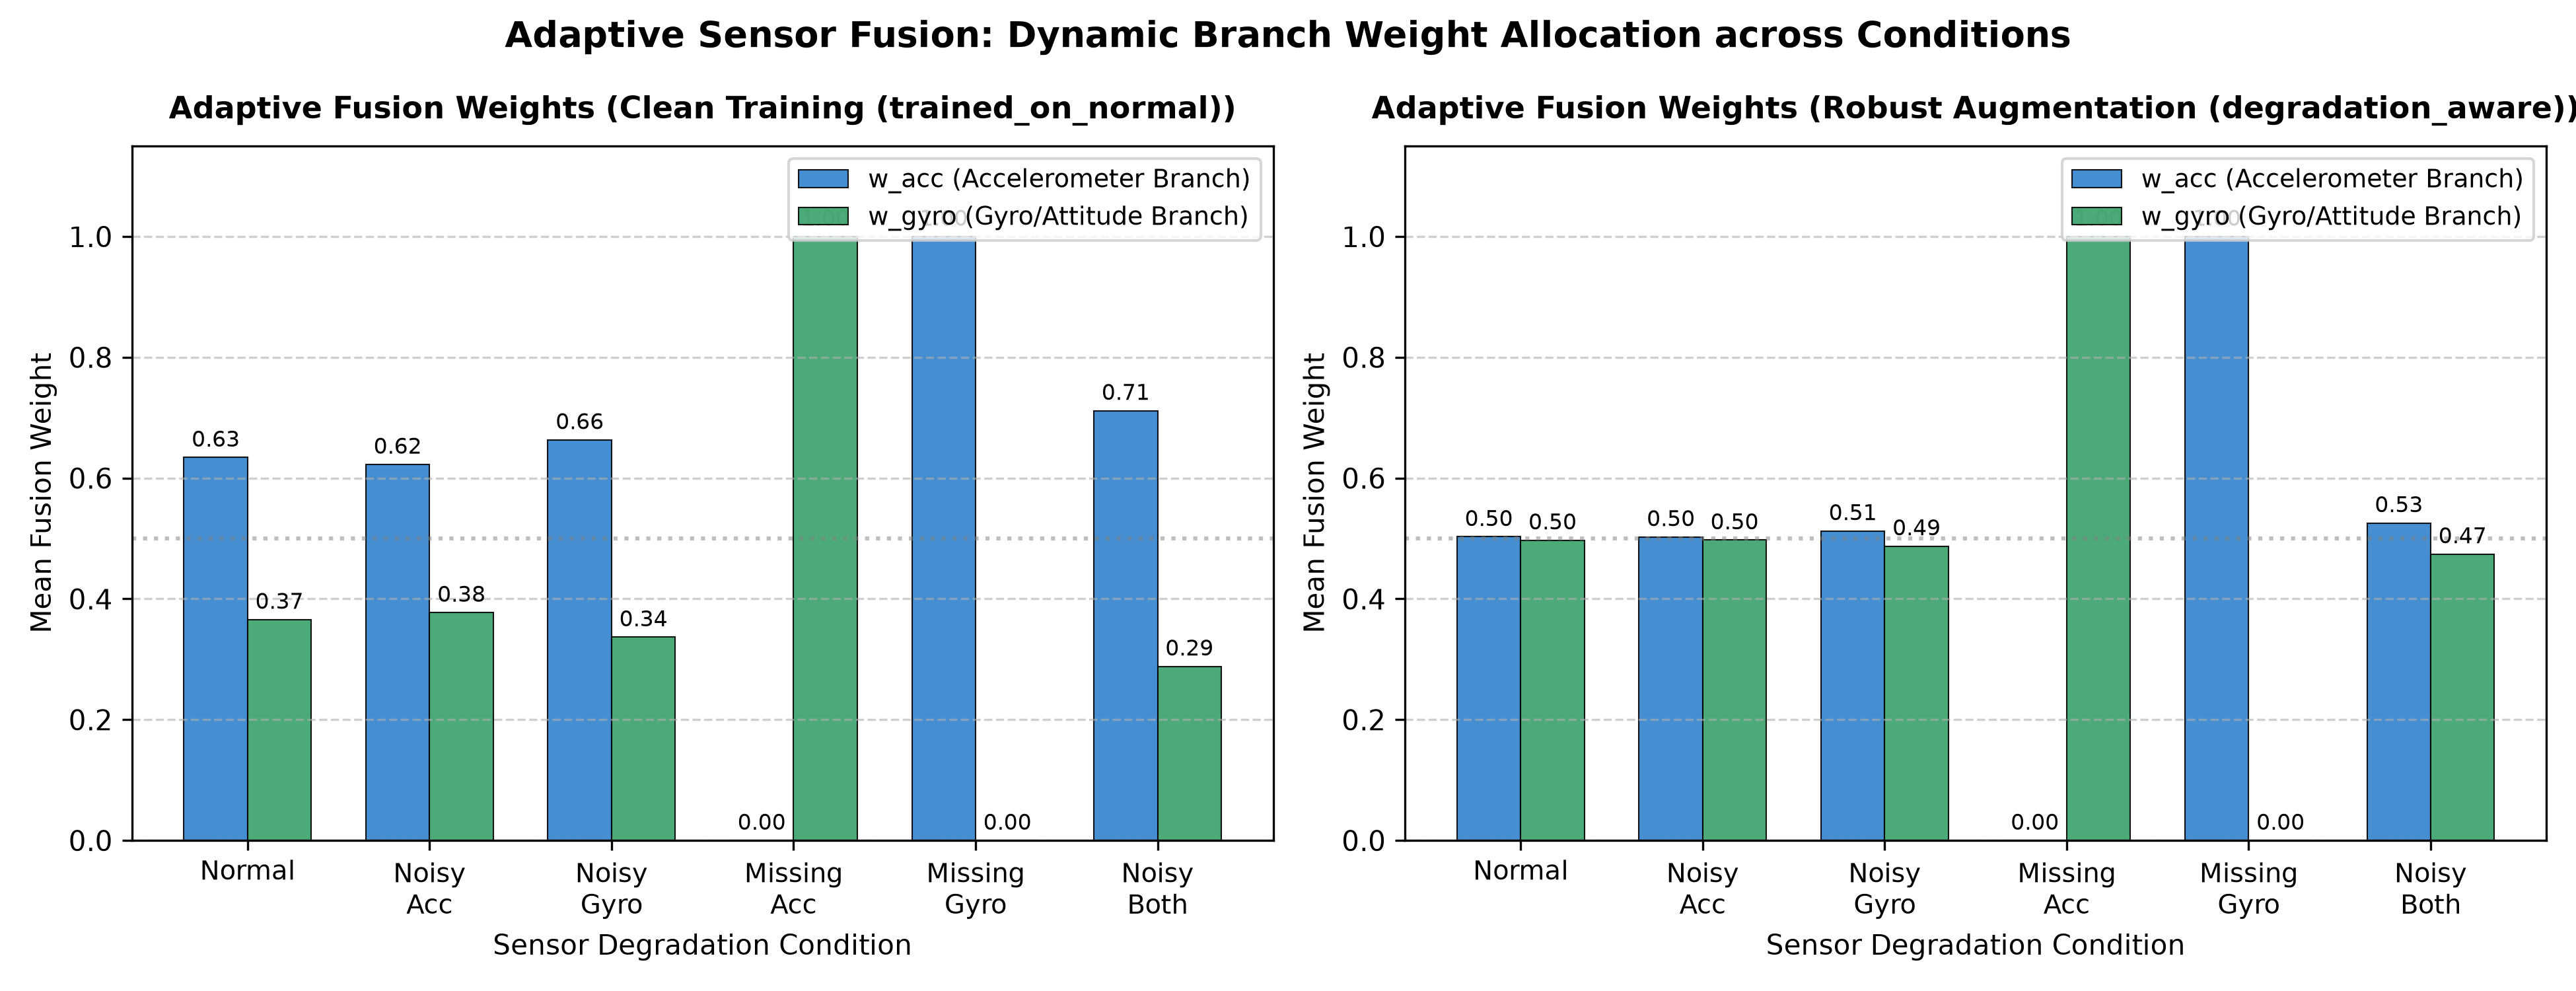
\includegraphics[width=0.88\linewidth]{results/adaptive_fusion_weights.png}
\caption{Dynamic Branch Weight Reallocation ($w_{\text{acc}}$ vs. $w_{\text{gyro}}$) Computed by AdaptiveFusionModule across Sensor Degradation Conditions.}
\label{fig:fusion_weights}
\end{figure}

As evidenced by Table~\ref{tab:degradation_results}, Table~\ref{tab:adaptive_weights_summary}, and Figure~\ref{fig:fusion_weights}, when an entire modality is disconnected (\texttt{missing\_acc} or \texttt{missing\_gyro}), \texttt{AdaptiveSensorFusion} successfully dynamically reallocates 100\% of fusion weight to the operational modality. Detailed comparative observations between architectures are discussed in subsequent sections.

% ----------------------------------------------------------------------------
% Subsection 8: Limitations
% ----------------------------------------------------------------------------
\subsection{Methodological and Experimental Limitations}
\label{subsec:limitations}

While our experimental pipeline enforces strict leakage-free data partitioning and reproducible degradation modeling, several methodological limitations must be acknowledged:
\begin{enumerate}
    \item \textbf{Synthetic vs. Physical Hardware Degradation:} Our degradation protocol simulates sensor failure through zero-fill masking and additive Gaussian perturbations. In operational mobile devices, hardware degradation often exhibits non-linear phenomena, including sensor bias drift, analog-to-digital clipping, temperature-induced calibration offsets, and intermittent sampling jitter, which are not fully captured by independent Gaussian distributions.
    \item \textbf{Cohort Size and Subject Diversity:} The MotionSense dataset comprises 24 total participants performing scripted trials. Although subject-wise partitioning eliminates identity contamination, the 4-participant test cohort ($N_{\text{test}} = 4$) represents a relatively small sample of human physiological diversity. Inter-subject variations in device placement, body mass index (BMI), and walking cadence can introduce variance in holdout test metrics.
    \item \textbf{Single-Device Placement Assumption:} MotionSense records motion from a smartphone positioned exclusively in the front right trouser pocket. Consequently, learned representations reflect thigh kinematic profiles. Real-world HAR applications must contend with arbitrary device placement (e.g., backpacks, hand-held texting, armbands), requiring multi-position evaluation in future work.
\end{enumerate}

